% Options for packages loaded elsewhere
% Options for packages loaded elsewhere
\PassOptionsToPackage{unicode}{hyperref}
\PassOptionsToPackage{hyphens}{url}
\PassOptionsToPackage{dvipsnames,svgnames,x11names}{xcolor}
%
\documentclass[
  british,
  a4paper,
]{article}
\usepackage{xcolor}
\usepackage{amsmath,amssymb}
\setcounter{secnumdepth}{-\maxdimen} % remove section numbering
\usepackage{iftex}
\ifPDFTeX
  \usepackage[T1]{fontenc}
  \usepackage[utf8]{inputenc}
  \usepackage{textcomp} % provide euro and other symbols
\else % if luatex or xetex
  \usepackage{unicode-math} % this also loads fontspec
  \defaultfontfeatures{Scale=MatchLowercase}
  \defaultfontfeatures[\rmfamily]{Ligatures=TeX,Scale=1}
\fi
\usepackage{lmodern}
\ifPDFTeX\else
  % xetex/luatex font selection
\fi
% Use upquote if available, for straight quotes in verbatim environments
\IfFileExists{upquote.sty}{\usepackage{upquote}}{}
\IfFileExists{microtype.sty}{% use microtype if available
  \usepackage[]{microtype}
  \UseMicrotypeSet[protrusion]{basicmath} % disable protrusion for tt fonts
}{}
\makeatletter
\@ifundefined{KOMAClassName}{% if non-KOMA class
  \IfFileExists{parskip.sty}{%
    \usepackage{parskip}
  }{% else
    \setlength{\parindent}{0pt}
    \setlength{\parskip}{6pt plus 2pt minus 1pt}}
}{% if KOMA class
  \KOMAoptions{parskip=half}}
\makeatother
% Make \paragraph and \subparagraph free-standing
\makeatletter
\ifx\paragraph\undefined\else
  \let\oldparagraph\paragraph
  \renewcommand{\paragraph}{
    \@ifstar
      \xxxParagraphStar
      \xxxParagraphNoStar
  }
  \newcommand{\xxxParagraphStar}[1]{\oldparagraph*{#1}\mbox{}}
  \newcommand{\xxxParagraphNoStar}[1]{\oldparagraph{#1}\mbox{}}
\fi
\ifx\subparagraph\undefined\else
  \let\oldsubparagraph\subparagraph
  \renewcommand{\subparagraph}{
    \@ifstar
      \xxxSubParagraphStar
      \xxxSubParagraphNoStar
  }
  \newcommand{\xxxSubParagraphStar}[1]{\oldsubparagraph*{#1}\mbox{}}
  \newcommand{\xxxSubParagraphNoStar}[1]{\oldsubparagraph{#1}\mbox{}}
\fi
\makeatother


\usepackage{longtable,booktabs,array}
\newcounter{none} % for unnumbered tables
\usepackage{calc} % for calculating minipage widths
% Correct order of tables after \paragraph or \subparagraph
\usepackage{etoolbox}
\makeatletter
\patchcmd\longtable{\par}{\if@noskipsec\mbox{}\fi\par}{}{}
\makeatother
% Allow footnotes in longtable head/foot
\IfFileExists{footnotehyper.sty}{\usepackage{footnotehyper}}{\usepackage{footnote}}
\makesavenoteenv{longtable}
\usepackage{graphicx}
\makeatletter
\newsavebox\pandoc@box
\newcommand*\pandocbounded[1]{% scales image to fit in text height/width
  \sbox\pandoc@box{#1}%
  \Gscale@div\@tempa{\textheight}{\dimexpr\ht\pandoc@box+\dp\pandoc@box\relax}%
  \Gscale@div\@tempb{\linewidth}{\wd\pandoc@box}%
  \ifdim\@tempb\p@<\@tempa\p@\let\@tempa\@tempb\fi% select the smaller of both
  \ifdim\@tempa\p@<\p@\scalebox{\@tempa}{\usebox\pandoc@box}%
  \else\usebox{\pandoc@box}%
  \fi%
}
% Set default figure placement to htbp
\def\fps@figure{htbp}
\makeatother



\ifLuaTeX
\usepackage[bidi=basic,shorthands=off]{babel}
\else
\usepackage[bidi=default,shorthands=off]{babel}
\fi
\ifLuaTeX
  \usepackage{selnolig} % disable illegal ligatures
\fi


\setlength{\emergencystretch}{3em} % prevent overfull lines

\providecommand{\tightlist}{%
  \setlength{\itemsep}{0pt}\setlength{\parskip}{0pt}}



 


\makeatletter
\@ifpackageloaded{tcolorbox}{}{\usepackage[skins,breakable]{tcolorbox}}
\@ifpackageloaded{fontawesome5}{}{\usepackage{fontawesome5}}
\definecolor{quarto-callout-color}{HTML}{909090}
\definecolor{quarto-callout-note-color}{HTML}{0758E5}
\definecolor{quarto-callout-important-color}{HTML}{CC1914}
\definecolor{quarto-callout-warning-color}{HTML}{EB9113}
\definecolor{quarto-callout-tip-color}{HTML}{00A047}
\definecolor{quarto-callout-caution-color}{HTML}{FC5300}
\definecolor{quarto-callout-color-frame}{HTML}{acacac}
\definecolor{quarto-callout-note-color-frame}{HTML}{4582ec}
\definecolor{quarto-callout-important-color-frame}{HTML}{d9534f}
\definecolor{quarto-callout-warning-color-frame}{HTML}{f0ad4e}
\definecolor{quarto-callout-tip-color-frame}{HTML}{02b875}
\definecolor{quarto-callout-caution-color-frame}{HTML}{fd7e14}
\makeatother
\makeatletter
\@ifpackageloaded{caption}{}{\usepackage{caption}}
\AtBeginDocument{%
\ifdefined\contentsname
  \renewcommand*\contentsname{Table of contents}
\else
  \newcommand\contentsname{Table of contents}
\fi
\ifdefined\listfigurename
  \renewcommand*\listfigurename{List of Figures}
\else
  \newcommand\listfigurename{List of Figures}
\fi
\ifdefined\listtablename
  \renewcommand*\listtablename{List of Tables}
\else
  \newcommand\listtablename{List of Tables}
\fi
\ifdefined\figurename
  \renewcommand*\figurename{Figure}
\else
  \newcommand\figurename{Figure}
\fi
\ifdefined\tablename
  \renewcommand*\tablename{Table}
\else
  \newcommand\tablename{Table}
\fi
}
\@ifpackageloaded{float}{}{\usepackage{float}}
\floatstyle{ruled}
\@ifundefined{c@chapter}{\newfloat{codelisting}{h}{lop}}{\newfloat{codelisting}{h}{lop}[chapter]}
\floatname{codelisting}{Listing}
\newcommand*\listoflistings{\listof{codelisting}{List of Listings}}
\makeatother
\makeatletter
\makeatother
\makeatletter
\@ifpackageloaded{caption}{}{\usepackage{caption}}
\@ifpackageloaded{subcaption}{}{\usepackage{subcaption}}
\makeatother
\usepackage{bookmark}
\IfFileExists{xurl.sty}{\usepackage{xurl}}{} % add URL line breaks if available
\urlstyle{same}
% fallback for those not using the hyperref driver hyperxmp:
\makeatletter
\@ifundefined{xmpquote}{\newcommand{\xmpquote}[1]{#1}}{}
\makeatother
\hypersetup{
  pdftitle={Inflation forecasts as probabilities{,} not single numbers},
  pdfauthor={Carlos Galindo},
  pdflang={en-GB},
  colorlinks=true,
  linkcolor={blue},
  filecolor={Maroon},
  citecolor={Blue},
  urlcolor={Blue},
  pdfcreator={LaTeX via pandoc}}


\title{Inflation forecasts as probabilities, not single numbers}
\usepackage{etoolbox}
\makeatletter
\providecommand{\subtitle}[1]{% add subtitle to \maketitle
  \apptocmd{\@title}{\par {\large #1 \par}}{}{}
}
\makeatother
\subtitle{A monthly forecast pack for 22 economies that pools
independent views of the next print and the year ahead into one
distribution, and reads it as the odds of crossing the thresholds that
matter}
\author{Carlos Galindo}
\date{}
\begin{document}
\maketitle


\begin{tcolorbox}[enhanced jigsaw, arc=.35mm, bottomrule=.15mm, breakable, colback=white, colframe=quarto-callout-note-color-frame, left=2mm, leftrule=.75mm, opacityback=0, rightrule=.15mm, toprule=.15mm]

\vspace{-3mm}\textbf{At a glance}\vspace{3mm}

\begin{itemize}
\tightlist
\item
  \textbf{Question.} What are the odds that inflation ends up above, or
  below, the levels that matter to a central bank, an investor or a
  budget, next month and a year from now?
\item
  \textbf{Approach.} For each economy and each month, a forecast pack
  that pools several independent views into one distribution of
  outcomes, keeps that distribution's real shape, and reads it as
  probabilities.
\item
  \textbf{Finding.} The pack runs for headline and core inflation across
  22 economies. Each edition gives a full distribution at four horizons,
  the probability of exceeding any threshold, the odds of staying in a
  high-inflation regime, and scenario paths for the exchange rate and
  energy prices.
\item
  \textbf{Why it matters.} A single forecast number hides the risks that
  drive decisions. Probabilities of crossing a threshold are what a
  policy committee, a portfolio manager or a fiscal planner can act on
  directly.
\end{itemize}

\end{tcolorbox}

\subsection{The question}\label{the-question}

Most inflation forecasts arrive as one number. Decisions rarely turn on
one number. A central bank cares whether inflation will be back inside
its target band; a bond investor cares about the chance of an upside
surprise next month; a finance ministry cares about the odds that
indexation costs overshoot the budget. Each of these is a question about
probabilities, and each needs the whole distribution of outcomes,
including its lopsided tails.

The difficulty is that inflation distributions are often not
bell-shaped. After a large shock, an economy can sit between two
regimes: a path back to normal, and a path where high inflation
persists. Administered prices, tax changes and energy pass-through add
discrete jumps. A forecast that assumes a symmetric bell curve misses
exactly the risks a reader most needs to see.

This project rebuilt and improved the probabilistic layer of a
multi-country inflation projection system that was begun in a previous
role. The aim is one consistent forecast pack per economy per month,
readable as odds rather than as a single line.

\subsection{Approach}\label{approach}

\subsubsection{Several independent views of the same
outcome}\label{several-independent-views-of-the-same-outcome}

Each edition forms three views of the coming months, each built
differently:

\begin{itemize}
\tightlist
\item
  a \textbf{fundamentals view}, driven by the economy's own inflation
  dynamics and a composite of the external and domestic drivers that
  move with inflation over the long run, such as the exchange rate,
  energy prices, activity and financial conditions;
\item
  a \textbf{regime-aware view}, which allows for distinct inflation
  regimes and for jumps between them, so that a minority high-inflation
  outcome is kept rather than averaged away;
\item
  a \textbf{structured judgement view}, which brings in informed priors
  about the next print in a disciplined, repeatable form.
\end{itemize}

\subsubsection{Pooling the views and keeping their
shape}\label{pooling-the-views-and-keeping-their-shape}

The three views are pooled into one combined distribution. None of them
is forced into a bell curve first, so the combined distribution keeps
every peak and tail the evidence supports. When the views agree, it is
narrow and single-peaked. When they disagree, it shows two or more
peaks, and the disagreement itself becomes visible information rather
than being blurred into a wider bell curve.

\subsubsection{Reading the distribution}\label{reading-the-distribution}

Each edition then turns the distribution into readings a decision-maker
can use directly:

\begin{enumerate}
\def\labelenumi{\arabic{enumi}.}
\tightlist
\item
  \textbf{Balance of risks at four horizons:} next month, twelve months,
  eighteen months and the end of the following year.
\item
  \textbf{Threshold probabilities:} for every level of inflation, the
  probability that the outcome exceeds it, with a confidence band.
\item
  \textbf{Regime persistence:} the probability, month by month, of
  remaining in a high-inflation regime.
\item
  \textbf{Conditioning paths and scenarios:} the exchange-rate and
  energy assumptions behind the central path, and a grid of alternative
  paths in which each moves up or down.
\item
  \textbf{Underlying signal:} trend, seasonal and momentum readings of
  the latest data, so the starting point is clean before any forecast is
  made.
\item
  \textbf{An outside comparison:} the central path and its range, set
  against an independent external forecast.
\end{enumerate}

\subsection{What the work shows}\label{what-the-work-shows}

The first result is the pooled distribution. The figure shows the idea
on simulated data: three views of next month's price change, one of them
with a small second peak for a jump scenario, and the combined
distribution that keeps that peak visible.

\begin{figure}

\centering{

\pandocbounded{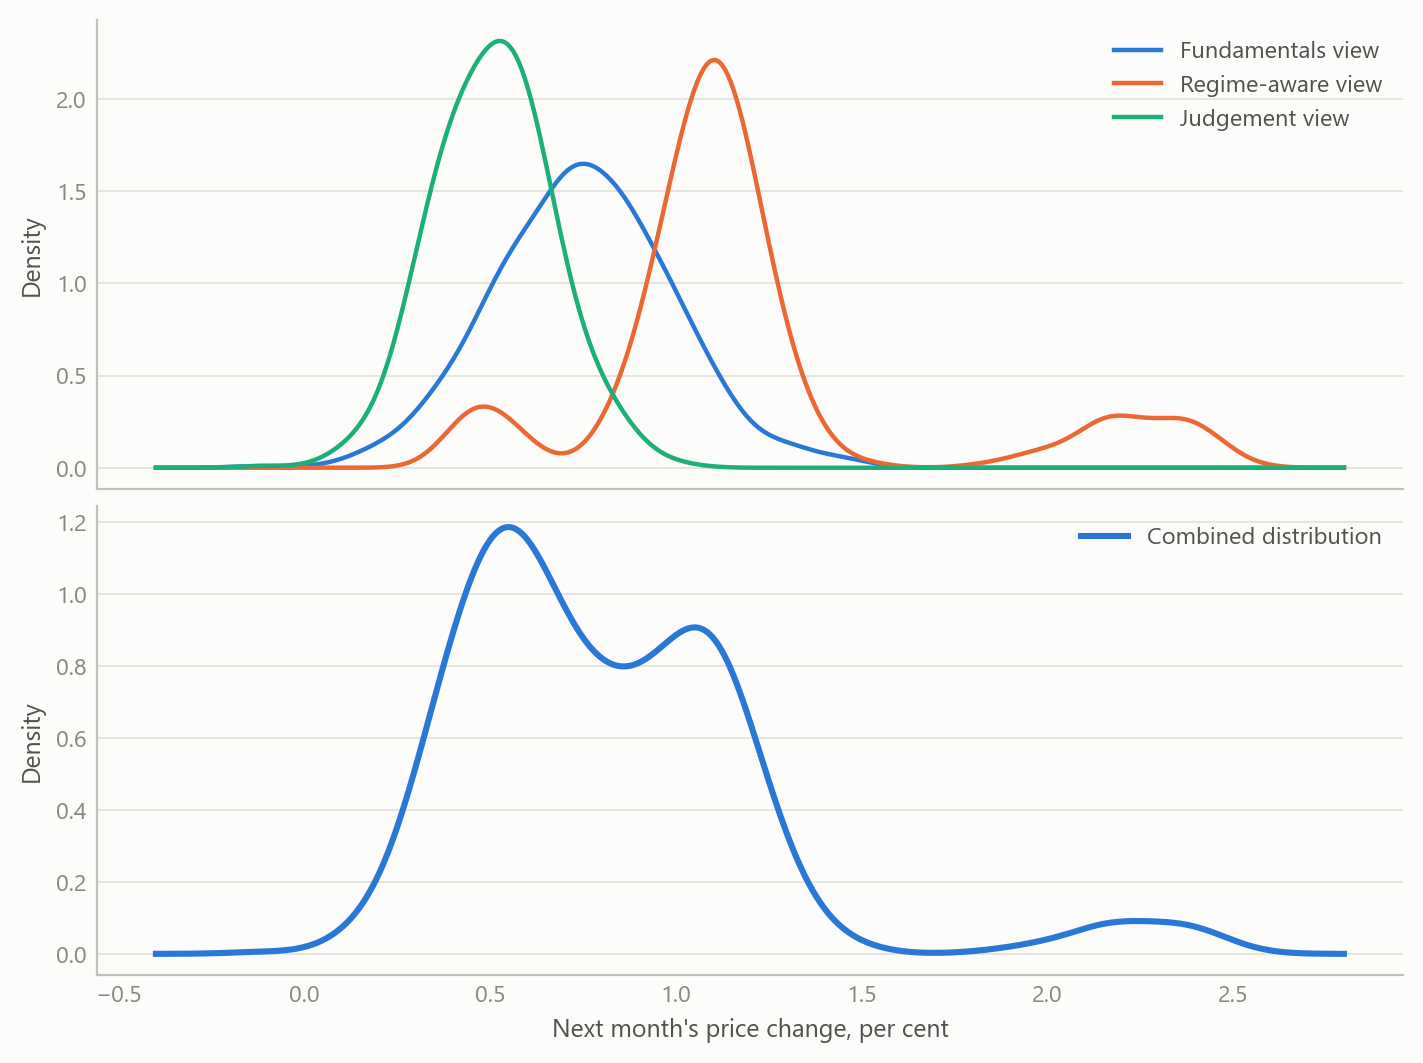
\includegraphics[keepaspectratio]{index_files/figure-latex/fig-views-output-1.png}}

}

\caption{\label{fig-views}Three independent views of next month's price
change (top) pooled into one combined distribution (bottom) (simulated
data).}

\end{figure}%

The second result is the reading in probabilities. The curve below
gives, for each level of inflation a year ahead, the probability that
the outcome exceeds it. A reader picks the threshold that matters to
them, such as the top of a target band, and reads off the odds.

\begin{figure}

\centering{

\pandocbounded{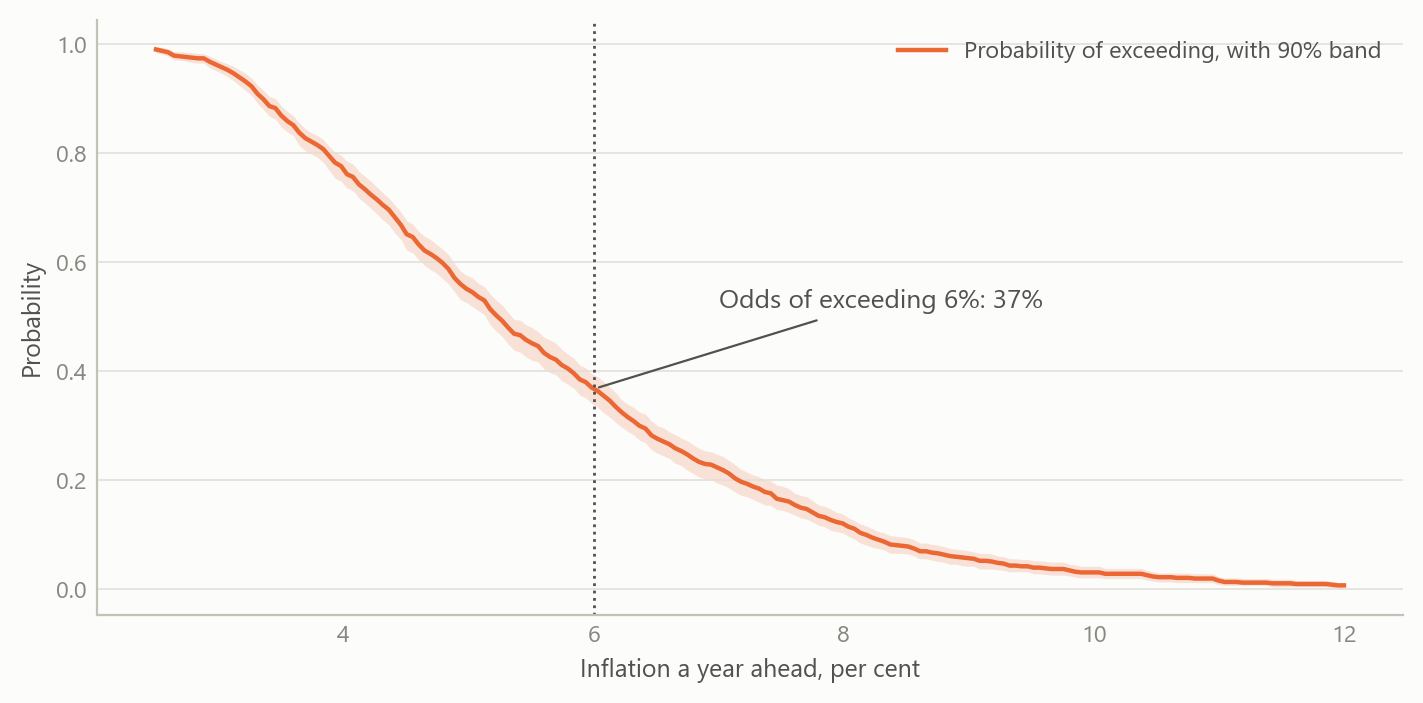
\includegraphics[keepaspectratio]{index_files/figure-latex/fig-survival-output-1.png}}

}

\caption{\label{fig-survival}Probability that inflation a year ahead
exceeds each level, with a 90 per cent confidence band (simulated
data).}

\end{figure}%

The third result is the balance of risks across horizons. The same pack
shows how the range of outcomes widens with the horizon, and whether the
risks lean up or down at each one.

\begin{figure}

\centering{

\pandocbounded{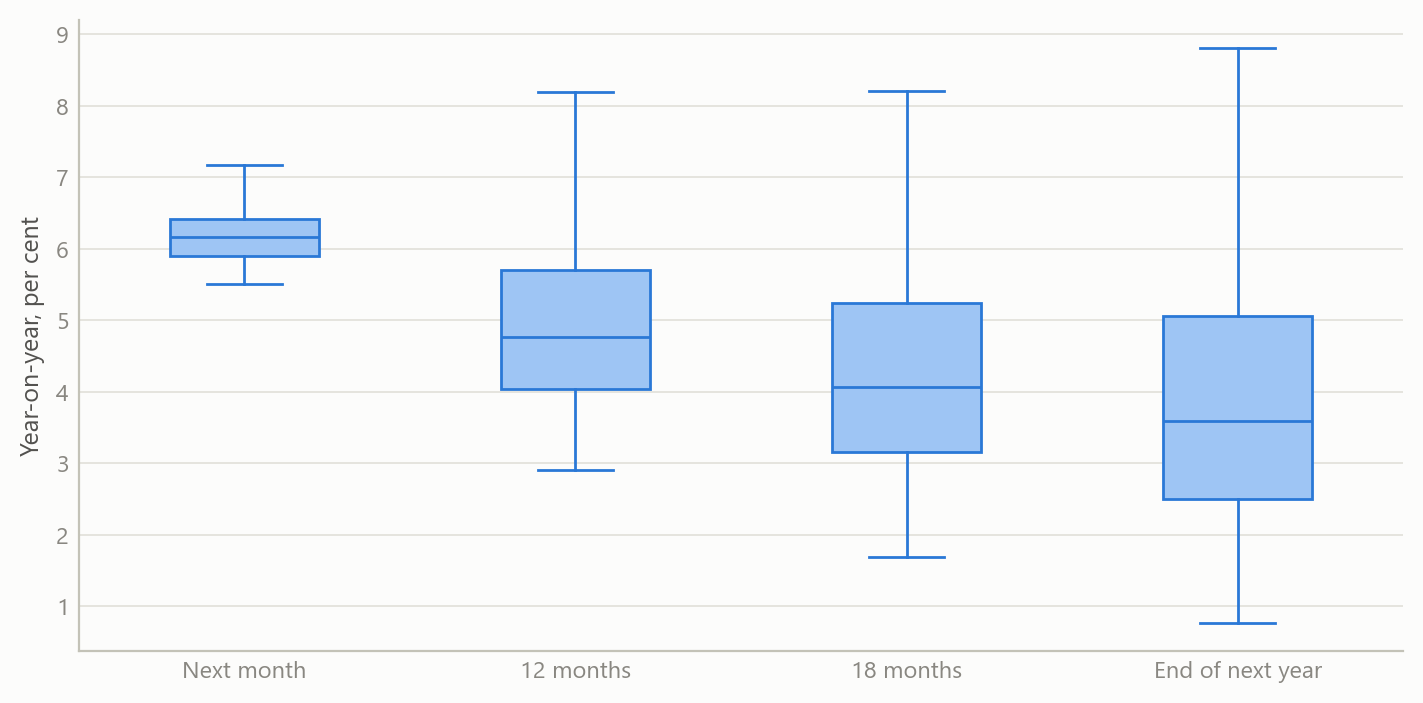
\includegraphics[keepaspectratio]{index_files/figure-latex/fig-risks-output-1.png}}

}

\caption{\label{fig-risks}Balance of risks at four horizons: the spread
of outcomes widens, and its skew shows which way the risks lean
(simulated data).}

\end{figure}%

The fourth result is the scenario view. Starting from the end of a
high-inflation episode, the central path is shown with a grid of
alternatives in which the exchange rate and energy prices each move up
or down by a moderate or a large amount. The spread of the paths shows
how much of the outlook rests on those two assumptions.

\begin{figure}

\centering{

\pandocbounded{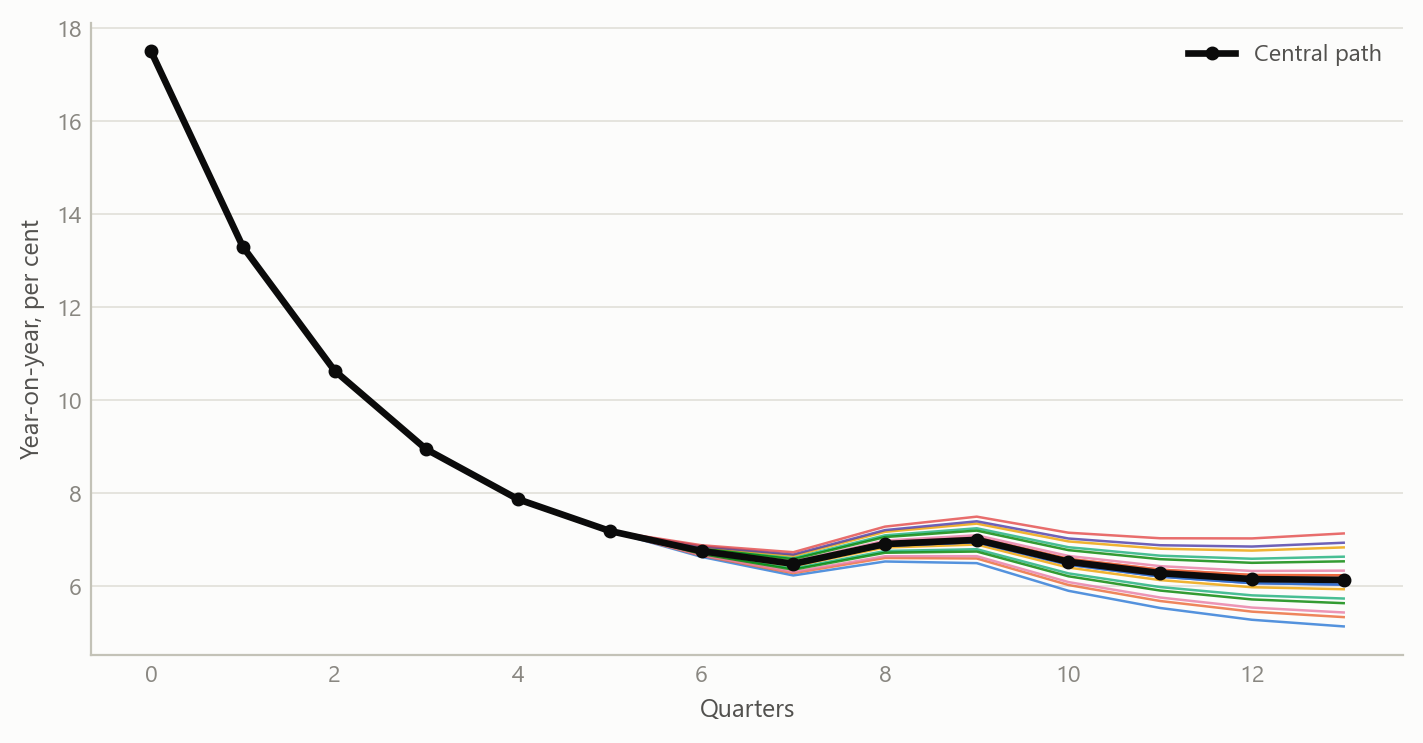
\includegraphics[keepaspectratio]{index_files/figure-latex/fig-scenarios-output-1.png}}

}

\caption{\label{fig-scenarios}Central path and sixteen alternative paths
from a grid of exchange-rate and energy-price shocks (simulated data).}

\end{figure}%

\subsection{Insights}\label{insights}

\begin{itemize}
\tightlist
\item
  \textbf{Odds are the product.} Turning a forecast into the probability
  of crossing a threshold answers the question decision-makers actually
  ask, and makes forecasts from different economies directly comparable.
\item
  \textbf{Keep the shape.} Pooling views without forcing them into a
  bell curve lets a minority scenario, such as a jump in administered
  prices or a stalled disinflation, stay visible as a second peak
  instead of disappearing into an average.
\item
  \textbf{Disagreement is information.} When independent views point in
  different directions, the combined distribution shows it at a glance.
  That is often the most useful signal in a month's edition.
\item
  \textbf{Regimes matter most at turning points.} The probability of
  staying in a high-inflation regime is the reading that moves first
  when an episode ends, and it gives an early, quantified answer to ``is
  it over?''.
\item
  \textbf{One pack, many economies.} Producing the same readings every
  month for 22 economies turns a set of country forecasts into a
  consistent cross-country view of risk.
\end{itemize}

\subsection{Scope and next steps}\label{scope-and-next-steps}

The pack is built for economies where inflation risks are lopsided:
after large shocks, under administered prices, and wherever the exchange
rate and energy prices pass through quickly. It runs for headline and
core inflation, with monthly editions continuing to January 2025.

The natural extensions are three. First, scoring the distributions over
time with probability-based measures, so that each view's weight can be
learned from its record. Second, adding market-implied and survey-based
views as further independent inputs. Third, publishing the threshold
probabilities as a compact cross-country dashboard.

The full method and worked examples from real editions can be discussed
on request.

\subsection{About the evidence}\label{about-the-evidence}

The work rebuilt and improved a system begun in a previous role. Monthly
editions cover headline and core inflation for 22 economies, each with
forecast distributions, threshold probabilities, regime probabilities
and a balance of risks. The most recent editions run to January 2025.
All figures on this page are simulated and illustrate the method only.

Figures and tables marked \emph{simulated} are generated from simulated
data built to share the structure of the analysis (its variables,
horizons and frequencies). They show how each method works and what its
output looks like. Results stated in the text, and figures that give a
source, are the project's own. Methods are described at the level of a
methods section. Code and data pipelines are not reproduced here.




\end{document}
